\cleardoublepage
\appendix

\chapter{Logging practice in software engineering}\label{apx:loggingPractice}
Providing a guide for software engineers and developers to implement a suitable logging mechanism in their software systems has proven to be a vital tool for both industrial use and academic progress \cite{Rong2018a}. Guoping Rong et al. conducted a study to review published papers on logging practices and improve the performance and efficiency of logging implementation. From their study, they established selection criteria for including (as in \Cref{tbl:CH1_RongIncSelectionCriteria}) and excluding (as in \Cref{tbl:CH1_RongExlSelectionCriteria}) academic papers about logging practices \cite{Rong2018a,Rong2018}.\par Rong's selection criteria yielded numerous research papers on logging practices applied in the industry, either through creating a new logging mechanism or optimizing existing logging mechanisms. By reviewing 41 identified papers, they found that many practitioners and researchers recognize the importance of logging practices in software engineering. However, there is a lack of guidance available to provide software engineers or developers with the necessary tools to create or improve efficient logging mechanisms \cite{Rong2018a,Zhu2015}.

\begin{table}[!htb]
	\centering
	\caption[G. Rong's inclusion selection criteria]
	{\textit{G. Rong's inclusion selection criteria \cite{Rong2018a}}}
	\label{tbl:CH1_RongIncSelectionCriteria}
	\begin{tabularx}{\textwidth}{|c|X|}
		\hline \textbf{Identification} & \textbf{Criteria} \\
		\hline I1. & Publications that investigate the methodology for logging practice. \\
		\hline I2. & Publications that investigate the tools, frameworks, systems which support logging practice. \\
		\hline I3. & Publications that propose a standard for logging practice.\\
		\hline I4. & Publications that are peer-reviewed (conference paper, journal article). \\
		\hline I5. & Publications that are primary studies on logging practice. \\
		\hline
	\end{tabularx}
\end{table}

\begin{table}[!htb]
	\centering
	\caption[G. Rong's exclusion selection criteria]
	{\textit{G. Rong's exclusion selection criteria \cite{Rong2018a}}}
	\label{tbl:CH1_RongExlSelectionCriteria}
	\begin{tabularx}{\textwidth}{|c|X|}
		\hline \textbf{Identification} & \textbf{Criteria} \\
		\hline E1. & Publications that investigate log analysis. \\
		\hline E2. & Publications that investigate the usage of logs. \\
		\hline E3. & Publications that investigate the technologies on logging user behaviours. \\
		\hline E4. & Publications that are not written in English. \\
		\hline E5. & Additionally, short papers, demo or industry publications are excluded. \\
		\hline
	\end{tabularx}
\end{table}

\clearpage

\Cref{fig:PushblisedPapers} shows the distribution of the 41 published papers obtained for Rong's research on logging practices. Event logging has an increasingly important role in modern software systems; therefore, research on logging practices in software engineering has been on the rise between 1990 and 2017.

\begin{figure}[!htb] % An h :here, t: top, b: bottom.
	\centering % cent the figure
	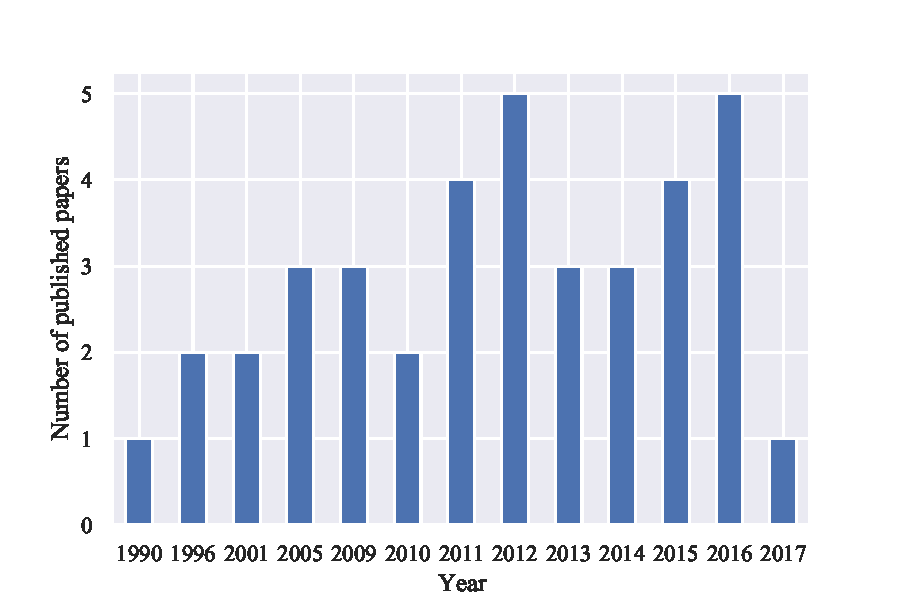
\includegraphics[width=0.95\textwidth]{Chapter1/Ronga2018.pdf}
	\caption[The distribution of the papers’ published years]
	{\textit{The distribution of the papers’ published years \cite{Rong2018a}}} \label{fig:PushblisedPapers}
\end{figure} 
